%  SingleXBs
%  Created by Dave Williams on 2009-06-25.
%  

% header (fold)
\documentclass[]{article}

\usepackage{setspace, float, fancyhdr}
\usepackage[pdftex]{graphicx}
\usepackage[utf8]{inputenc}
\usepackage[round,numbers,sort&compress]{natbib} 
\addtolength{\parskip}{\baselineskip}
\setlength{\parindent}{0in}

% Multipart figures
%\usepackage{subfigure}
% Package for including code in the document
%\usepackage{listings}

% FIXME: More descriptive title would be nice.
\title{Simple and complex multidimensional actomyosin crossbridges} 
\author{C.D.\ Williams, M.\ Regnier, T.L.\ Daniel}
\date{2009--06--25}
% header (end)

\begin{document}

\maketitle{}

\begin{abstract} 
Existing spatially explicit models of muscle contraction treat myosin as a single spring oriented parallel to the direction of contraction.
Here we describe a model of myosin that incorporates multiple springs, forming a four spring crossbridge (4sXB) that closely replicates the motions used in myosin's power stroke to generate force.
This 4sXB model is able to take most of its parameters from experimental measurements and permits monitoring of phenomena not possible with a single-spring crossbridge.
The 4sXB generates radial force (orthogonal to the direction of contraction) during its power stroke similar to what a physical crossbridge produces.
Also, as with physical crossbridges, the 4sXB's kinetics and force production vary with lattice spacing as angles of attachment, crossbridge geometry and diffusion distances change.
Additionally, we propose a simpler two spring crossbridge (2sXB) that replicates most qualities of the 4sXB.
Unlike the 4sXB, the length and angle of the springs comprising the 2sXB can be determined analytically for any chosen head position without the use of iterative techniques.
The forces generated by the 4sXB and the 2sXB are similar.
Both axial and radial forces generated by the multi-spring crossbridges increase in magnitude as lattice spacing is offset from the crossbridge head resting position.
Radial forces generated by both multi-spring crossbridges vary with lattice spacing but remain between \%20 and \%120 of axial forces.
\end{abstract}

Keywords: myosin; spatially-explicit model; crossbridge kinetics

% \paragraph*{Author Summary} % (fold)
% Models of muscle contraction have long treated the molecular motor myosin as a simple spring oriented parallel to its direction of movement. 
% This does not allow for the investigation of phenomena such as the perpendicular force observed during shortening, or the dependence of the maximum force produced on spacing between the contractile filaments that comprise muscle.
% We demonstrate an alternative model, computationally simple enough to use in large networked models, that incorporates both linear and torsional (angle dependent) springs. 
% This model type captures much of the behavior missing from single spring models of the crossbridge.
% paragraph author_summary (end)


\section{Introduction} %(fold)

% While individual crossbridges have been treated independently with spatial modeling, thermodynamic accounting has been introduced to the crossbridge kinetics, compliance introduced to the filaments, and multiple filaments have been arranged to mimic the lattice, the one dimensional nature of the crossbridge has continued to be used as a model of the mechanism of force generation.

Radial forces of the same order as axial force have been shown to exist in  contracting muscles \citep{Cecchi1990, Millman1998}. 
These forces, and radial lattice spacing, have been put forward as a possible regulator of force generation \citep{Fuchs2005}. 
At the same time, increases in our knowledge of myosin's structure have lead to the idea that myosin generates force through the action of a lever arm \citep{Rayment1993, Uyeda1996, Huxley2000}.
Myosin's lever arm generates the strain that accompanies the powerstroke via a change in the rest angle at which the lever is attached to S1 region \citep{Huxley2000, Houdusse:2001:p182}. 
This change in angle occurs at the converter region, a flexible area that and acts as a torsional or angular spring. 
It has been suggested that these phenomena are related, that radial forces during force generation by a crossbridge are a result of the geometry of the lever arm \citep{Schoenberg1980b}. 

Existing theoretical and computational models of crossbridge force generation, at the filamental level, have used one-dimensional crossbridge models. 
As a consequence these computational studies have confined themselves, from the early work of \citet{Huxley1957} to more recent models \citep{Daniel1998, Chase:2004:p204, Tanner:2007:pe115}, to forces aligned along the axes of the contractile filaments.  
From a computational standpoint, less attention has been paid to radial forces. 
Thus, the geometry of the single spring crossbridge has remained largely unchanged while the kinetics underlying transitions between force generating states have increased in complexity throughout subsequent work \citep{Pate1989, Daniel1998, Tanner:2007:pe115}.
Meanwhile, the lever arm mechanism of force generation by myosin suggests that inclusion of torsional springs in computational models would create a system that better reflects the underlying mechanisms of the powerstroke. 

In this paper we examine and compare two torsional spring based crossbridge models, both well suited for use in spatially explicit models of the half sarcomere. 
The first is a four spring crossbridge (4sXB) based upon the structure of the S1 and S2 regions of myosin II. 
Following this, we consider a two spring crossbridge (2sXB) that replicates many of the behaviors of the 4sXB while requiring fewer computational resources. 
We derive three state kinetic systems for each type of crossbridge from those used by prior models. 
We quantify the radial force produced by these isolated crossbridges and how such forces increase as lattice spacings expand.
We also look at how changes in lattice spacing affect the other properties of the isolated crossbridges, such as how the optimum axial location of an available actin site for binding, the powerstroke, and detachment shifts towards the base of the crossbridge as lattice spacing increases. 

The crossbridge models developed here, when included in spatially explicit multi-filament models of the half-sarcomere, will permit such models to investigate the effects of radial forces and lattice spacings for the first time. 
Such models will be able to contribute to the ongoing discussion about the role that radial forces, transmitted directly or through titin, and changes in lattice spacing play in the Frank-Starling mechanism and in the regulation of Ca$^{2+}$ sensitivity as lattice spacing and sarcomere length vary. % TODO : Split into two sentences? Cite?

% % \paragraph{Comparison to previous systems} % (fold)
% This discussion owes a debt to \citet{Schoenberg1980a} and \citet{Schoenberg1980b} which contain a proposal and analysis of several different types of crossbridges, primarily two spring crossbridges where the S2 arm is represented as a linear spring and the S2-S1 junction area is represented as a torsional spring. 
% This system requires iterative solution methods, as our four spring crossbridge does, but restrains the crossbridge to an area within one S1 length of the line in which the S2 segment is set.
% % paragraph comparison_to_previous_systems (end)

% section introduction (end)


\section{Materials and Methods}  % (fold)

We consider two crossbridge models meant to capture a range of mechanical behaviors suggested by the literature.  
Each, described more fully below, can be derived from a generalized crossbridge consisting of 4 springs:  two torsional springs and two linear springs (Fig \ref{fig_xb_types}).  
These are contrasted to the traditional one-dimensional single spring model of a crossbridge.

\subsection*{Geometry} % (fold)

\paragraph{Spring configurations} % (fold)
The simplest crossbridge model examined here is similar to those used previously, and consists of a single linear spring parallel to the axes of the thick and thin filaments.
As the forces this crossbridge generates are solely in the direction of shortening, it can be described as a one-dimensional crossbridge. 
This one spring crossbridge (1sXB) is, as described above, the current crossbridge model implemented in most computational analyses. 
The one-dimensional 1sXB is insensitive to changes in lattice spacing, and unable to account for radial forces generated during axial shortening.

Our generalized four spring crossbridge (4sXB) uses two linear and two torsional springs to represent the myosin head, as depicted in Fig \ref{fig_xb_types}D.
This allows the springs used in the model to closely correspond to pieces of the crossbridge.
Specifically the four springs correspond to the S2/rod attachment point, the S2 region, the S2/light chain domain (LCD) attachment point, and the LCD.
The use of multiple springs by the 4sXB also allow it to represent properties of the crossbridge that are only present in two dimensional space, in contrast to the one-dimensional 1sXB. 
The rest angle of the torsional spring linking the S2 domain and the LCD simulates the powerstroke by increasing during the transition from a weakly bound to a strongly bound state.
This two dimensionality allows the 4sXB to be embedded in a space that takes the distance between thick and thin filaments into account, introducing lattice spacing dependence.

The 2sXB uses one linear and one torsional spring to represent the myosin head, (Fig.~\ref{fig_xb_types}C).
This crossbridge is a simplified version of the 4sXB, retaining movement generated by a lever arm, but altering the length of the lever such that it can bridge the entire distance between the thick and thin filaments.
The parameters characterizing the 2sXB are chosen to match the step size and kinetics of the 2sXB to those of the 4sXB.

Parameters for both crossbridges are derived, where possible, from existing physical measurements.
Each linear spring (one in the 1sXB, two in the 4sXB and one in the 2sXB) requires a rest length and spring constant, while each torsional spring (two in the 4sXB and one in the 2sXB) requires a rest angle and spring constant.
The lengths and angles of the springs used for the 4sXB are chosen from tomographic reconstructions of in vivo S2 lengths and x-ray crystallographic reconstructions of the S1 fragment \citep{Taylor1999, Rayment1993}.
The rest length and angle of the 2sXB are set so that the tips of the 2sXB and 4sXB are in the same location before and after the powerstroke.

% Should include a bit on spring constant derivation from Pi hydrolysis energies 
% Consider including a table of parameter values?

% paragraph spring_configurations (end)

\paragraph{Calculation of lattice spacing} % (fold)
Throughout this paper, d$_{1,0}$ lattice spacing is derived from the geometry of the crossbridge and the lattice spacing having the smallest radial force. 
The model provides a measurement of spacing that is analogous to the in vivo surface-to-surface distance between the thick and thin filaments.
The d$_{1,0}$ spacing is calculated from the surface-to-surface lattice spacing as $\rm{d}_{1,0} = 1.5 (surface-to-surface + offset)$ where the offset accounts for d$_{1,0}$ being measured from the center of one thick filament to another \citep{Millman1998}.
The offset used to calculate d$_{1,0}$ is determined by designating the resting surface-to-surface lattice spacing of a crossbridge in the post-powerstroke state as the lattice spacing at which radial forces are neither compressive nor expansive.  
This offset becomes 6.90 when the neutral force d$_{1,0}$ lattice spacing is defined as 34 nm \citep{Brenner1991}. 
The surface-to-surface lattice spacings that correspond to the range of extreme d$_{1,0}$ spacings are then back-calculated and used to define the window of lattice spacings we examine \citep{Millman1998}. % TODO : This could be better if it had more references to ``typical'' lattice spacing papers
Thus the rest surface-to-surface spacing in the model, the lattice spacing at which radial forces are minimal and the geometry of the actomyosin lattice are sufficient to parameterize how lattice spacing is defined for the modeled crossbridges. 
% paragraph calculation_of_lattice_spacing (end)

\paragraph{Displacement and force generation} % (fold)
Based on earlier mechanical models of force generation (e.g.\ Pate and Cooke; Daniel et al; Tanner et al.) each crossbridge undergoes a distortion upon the hydrolysis of ATP to ADP.Pi.  
That distortion changes the effective rest length of the crossbridge by an amount proportional to the energy derived from the hydrolysis.  
Within the 1sXB, this distortion is accomplished by a change in the rest length of the crossbridge's spring, while the 4sXB and 2sXB represent the distortion with a change in the rest angle of a torsional spring, a process more closely replicating the lever-arm mechanism \citep{Reedy2000}.
Upon release of Pi, distortional strain energy drives force generation by the crossbridge, essentially appearing as a change in the rest length of the molecule.
% paragraph displacement_and_force_generation (end)

\paragraph{Calculation of spring lengths and angles} % (fold)
% Goal here is to clearly communicate the ways in which the spring compoments are calculated. This should go through: what each angle actually is (from where to where with what as the apex), calculation of angle for 4sXB, and calculation of angle for the 2sXB.
When the 1sXB is placed under strain such that the myosin head is horizontally offset from the thick filament attachment site relative to its resting position, the length of the 1sXB's spring is simple to find as it must completely span the head to thick filament attachment distance.
The lengths and angles of the springs in the 2sXB and 4sXB must take into account the radial distance they must cover as well.
The 2sXB may be analytically determined, as it has all spring values set by the choice of a head location, with arm length and angle given by $r(h_x, h_y)=(h_x^2 + h_y^2)^{1/2}$ and $\theta(h_x, h_y)=\arctan(h_y/h_x)$, respectively.
The 4sXB's greater number of degrees of freedom mean it requires iterative optimization to find the location of the distal torsional spring representing the link between the S2 and S1 regions when the crossbridge's head is moved to a new location.
We use a modification of Powell's ``dog-leg'' method, present in the SciPy package of computational tools \citep{SciPy}, to relax the location of the distal torsional spring to that which results in the lowest energy state of the 4sXB.
Once the distal torsional spring's location is known (as $(c_x, c_y)$), the angle of the proximal torsional spring and the lengths of the two linear springs are determined analytically.
The angle of the proximal torsional spring is given as $\phi(c_x, c_y)=\arctan(c_y/c_x)$, the length of the proximal linear spring as $\ell(c_x, c_y)=(c_x^2 + c_y^2)^{1/2}$, the angle of the distal torsional spring as $\theta(c_x, c_y, h_x, h_y) = \arctan((h_y-c_y)/(h_x-c_x)) + \pi - \phi(c_x, c_y)$, and the length of the distal linear spring as $r(c_x, c_y, h_x, h_y)=((h_x-c_x)^2 + (h_y-c_y)^2)$.
% paragraph calculation_of_spring_lengths_and_angles (end)
% subsection geometry (end)

\subsection*{Kinetics} % (fold)
% * Kinetics
%  - Three states
%  - Distortion sensitive
%  - Free energy in each state
%   = Liberation of energy by Pi hydrolysis
%  - Calculation of binding rate
%   = Perturbation of crossbridge head
%   = Probability of binding based on distance to binding site
%  - Powerstroke rate
%   = Distortion dependence
%  - Unbinding rate
%  - Calculation of reverse rates
We choose to use a simplified three state model of the crossbridge cycle \citep{Pate1989, Tanner:2007:pe115}. 
This simplified system directly links the crossbridge's kinetics to mechanics; the three kinetic states are directly comparable to the myosin configurations described in \citet{Houdusse:2000:p11238}.
A secondary benefit of a three state kinetics system is that it allows multiple-motor models which use our many-spring crossbridges to more easily compare their results to those from the aforementioned previous models.

The three states represented in our kinetics are (1) an unbound state (2) a loosely-bound state and (3) a tightly-bound force-generating state.
These states correspond to a Myosin-ADP-Pi state, an Actin-Myosin-ADP-Pi state, and an Actin-Myosin-ADP state (Fig. \ref{fig_xb_types}A).

The kinetics of both the two spring and the four spring models are strain dependent and are essentially transforms of the free energy landscapes experienced by the crossbridges in their different states.
These free energies are a function of the distortion necessary to move the point representing the crossbridge's head to the point where we presume a binding site to be.
Examples of these free energy landscapes are visible in figures \ref{fig_kinetics_contours}A and \ref{fig_kinetics_contours}B, with cuts through them at the rest lattice spacing visible in figure \ref{fig_kinetics_cuts}A.

The binding of both the two and four spring crossbridges is determined by Monte-Carlo simulation of their diffusion as a result of being perturbed by Boltzmann derived energy distributions. 
After a new head location is found, a binding probability is calculated that decreases exponentially with distance from the potential binding site. 
This probability is tested against a random number from a uniform distribution to determine if binding occurs.
This method is similar to that used by \citet{Tanner:2007:pe115}. 

\paragraph{Free energy in each state} % (fold)
The total energy, liberated by the hydrolysis of a $P_i$, available to a crossbridge depends on the concentrations of $ATP$, $ADP$ and $P_i$ and is given by $\Delta G = -\Delta G_{0,ATP} - \ln \frac{[ATP]}{[ADP] [P_i]}$. 
In weakly and strongly bound states a portion of that energy is available to the crossbridge, allowing the crossbridge at most 28\% (in the weakly bound state) or 68\% (in the strongly bound state) of $\Delta G$ for mechanical work (see efficiency factors $\alpha=0.28$ and $\eta=0.68$ below; \citet{Pate1989, Tanner:2007:pe115}).
The total free energy of a crossbridge in each state also depends on the strain that the crossbridge experiences from distortion upon binding.
Thus the total free energy is a linear combination of the strain-dependent and phosphate-dependent energy of the crossbridge in each state.
The free energy of the 4sXB system in each state is: 
%Energy of the four spring crossbridge
\begin{eqnarray}
\label{4sEnergy}
U_1(\phi,\ell,\theta,r) & = & 0 \nonumber \\
U_2(\phi,\ell,\theta,r) & = & \alpha \Delta G + \frac{k_\phi (\phi-\phi_0)^2 + k_\ell (\ell-\ell_0)^2 + k_\theta (\theta-\theta_0)^2 + k_r (r-r_0)^2}{2} \nonumber \\
U_3(\phi,\ell,\theta,r) & = & \eta \Delta G + \frac{k_\phi (\phi-\phi_0)^2 + k_\ell (\ell-\ell_0)^2 + k_\theta (\theta-\theta_1)^2 + k_r (r-r_0)^2}{2} \nonumber
\end{eqnarray}
The free energy of the 2sXB system in each state is: 
% Energy of the two spring crossbridge
\begin{eqnarray}
\label{2sEnergy}
	U_1(r,\theta) & = & 0 \nonumber \\
    U_2(r,\theta) & = & \alpha \Delta G + \frac{k_r (r - r_0)^2 + 
                        k_\theta (\theta - \theta_0)^2}{2} \nonumber \\
    U_3(r,\theta) & = & \eta \Delta G   + \frac{k_r (r - r_1)^2 + 
                        k_\theta (\theta - \theta_1)^2}{2} \nonumber
\end{eqnarray}
% paragraph free_energy_in_each_state(end)

\paragraph{Binding rate calculation} % (fold)
 % History and modern stuff
 % Binding depends on
 % Overview of steps
 %  - diffusion
 %  - attachment
Our binding algorithm is descended from \citet{Tanner:2007:pe115} but differs in two key ways: we treat binding as a two step process and our diffusion step works with any number of springs.
Binding depends on diffusion of the crossbridge head and proximity to the nearest binding site.
Analogously, the process we use to simulate binding has two components, first the diffusion of the myosin head to a new location and then possible attachment to the nearest binding site (depending on the distance from the head and the binding site).
The first step, diffusion, is simulated by thermally forcing each of a crossbridge's constituent springs with an energy plucked from a Boltzman distribution.
This translates to assigning each spring a length or angle chosen from the probability density function $P(x) = \sqrt{k / (2 \pi kT)} \exp^{-(k x^2)/(2 kT)}$ where $x$ is the offset, $k$ is the spring constant of the spring under consideration, and $T$ is the system's temperature in Kelvin.
We find the updated location of the crossbridge head from these new spring lengths and angles.
% Probability of binding based on distance to binding site
The probability the crossbridge will form an attachment depends on the exponential of $d$, the distance from the crossbridge head's new location to the nearest binding site.
Specifically, the probability of attachment is given by $p_{12}(d) = \gamma \exp ^{d}$, where $\gamma$ is a scaling factor chosen to provide attachment rates consistent with previous estimates.
Attachment occurs if $p_{12}$ is greater than $rand$, a number between 0 and 1 chosen from a uniform distribution.
This process is used to determine whether a crossbridge binds during a single timestep; binding rates are calculated as the fraction of an ensemble of crossbridges that bind given the same starting conditions. 
Thus, for an ensemble of size $n$: 
$$r_{12} =  \frac{\sum_0^n \left( 1\; \textrm{if}\; \gamma \exp^{-d}>rand ,\; \textrm{else}\; 0 \right)}{n}$$
This two step system, with diffusion followed by a chance of attachment, is used for both the 4sXB and 2sXB with only a change in the number of thermally forced springs.
% paragraph binding_rate_calculation (end)

\paragraph{Powerstroke and detachment rates} % (fold)
% Distortion dependence
The powerstroke and detachment rates are based on the earlier work of \citet{Pate1989} and \citet{Tanner:2007:pe115}, and generalized here for the 4sXB and 2sXB in two-dimensional space. 
Both the powerstroke rate, $r_{23}$, and the detachment rate, $r_{31}$, are distortion dependent as they contain a term based on the differences in free energy between the current state and the one being considered for transition. 
This means that transitions are more likely when they are energetically favorable and less likely in other circumstances, a natural scheme based in the geometry of the crossbridges.
The particular rates are as follows for both the 4sXB and the 2sXB:
$$r_{23}(U_2, U_3) = 0.001 + 0.5 * (1 + \tanh(0.6 (U_2 - U_3))) $$
$$r_{31}(U_3, U_1) = e^{-1 / (U_3 - U_1)}$$
% paragraph unbinding_rate (end)

\paragraph{Calculation of reverse rates} % (fold)
% Technique of reverse rate calculation
Reverse transition rates are given by the thermodynamically balancing formula $r_{ij}/r_{ji}=\exp^{U_i-U_j}$ where $r_{ji}$ is the forward rate and $r_{ij}$ is the reverse rate (see \citet{Pate1989, Daniel1998, Tanner:2007:pe115}).
For the transition from a weakly bound state to an unbound state this requires that the reverse transition is again treated as a fraction of an ensemble of transition opportunities.
% paragraph calculation_of_reverse rates (end)
% subsection kinetics (end)

% section materials_and_methods (end)


\section{Results} % (fold)

% Results outline (fold)
 % Results:
 %  * Axial shifts of XBs' properties (e.g. maxs, mins) are tuned with lattice spacing
 %  * Magnitudes vary with lattice spacing
 %   - With exception of powerstroke rates
 %   - Powerstroke rates compare two parabolic energy profiles
 %  * Kinetics at rest lattice spacings are similar to previous efforts
 %   - Results of models using such systems can be compared to prior work
 %  * Radial forces 
 %   - Are on same order as axial forces
 %   - Depends on lattice spacing
 %   - Depends on axial offset
 %  * Axial forces
 %   - Levels depend on axial offset
 %   - But not so dependent on lattice spacing
% Results outline (end)

% Intro paragraph (fold)
The models we present here were developed to examine consequences of lattice spacing on crossbridge kinetics and two dimensional force production.
Multi-spring crossbridges introduce lattice spacing dependence into force production and kinetics, and account for forces not aligned with the direction of contraction.
As lattice spacing changes, the kinetics and forces of the 4sXB and 2sXB shift in either or both magnitude and axial offset.

\subparagraph{Axial offsets, magnitudes, axial components and radial components} % (fold)
The axial component of vector values, such as force, is the vector portion that lies along the axis of the thick and thin filaments.
The radial component of a vector value lies perpendicular to the thick and thin filaments, orthogonal to the axial component.
% subparagraph axial_offsets_magnitudes_axial_components_and_radial_components (end)

Baseline value changes occur where the lowest points, the highest points, or simply the offset of a value is shifted with regard to that seen at rest lattice spacing.
Baseline value changes manifest in, e.g., the lowered probability of any binding occurring at extreme lattice spacings. 
Key value offsets occur when maxima, minima, inflection points, or other landmarks of a value's profile are shifted axially from where they occur at rest lattice spacings.
Key value offsets are reflected in phenomena such as the axial offset at which a powerstroke will occur becoming right shifted at higher lattice spacings for the 2sXB.
In addition to these lattice spacing dependencies, we examine the ability of the 4sXB and the 2sXB to model the radial component of the force produced during the powerstroke.
% Intro paragraph (end)

\paragraph{At 34 nm $d_{10}$, the multi- and single-spring crossbridges have similar kinetics and energies} % (fold)
The free energy, binding rates, powerstroke rates and detachment rates of the 4sXB and 2sXB at a lattice spacing of 34 nm $d_{10}$ are similar to those of the 1sXB (Figure \ref{fig_kinetics_cuts}). 
This is because the kinetics and energies of the multi-spring crossbridges are derived from those of the single-spring crossbridge. 
The single-spring crossbridge kinetics and energies were modified to be independent of the number of springs in a crossbridge, instead depending on the free energy of the crossbridge head in its current location. 
The crossbridge properties of the 1sXB, 2sXB and 4sXB are shown together in figure \ref{fig_kinetics_cuts}, where the 1sXB values used are calculated as in figure 10 of \citet{Tanner:2007:pe115}. 
Although the properties of the multi- and single-spring crossbridges are largely similar, some divergences do occur. 
The multi-spring crossbridges' binding rate is a wider distribution than the single-spring crossbridge's binding rate due to the multi-spring crossbridges' use of diffusion-based binding probabilities.
This causes the 2sXB and 4sXB, when averaged over all offsets, to be less likely to bind but also to be more likely to bind at offsets with larger strains. 
The detachment rate of the single-spring crossbridge is its least energy-based value and required the most modification to function for all spring-based crossbridges. 
The detachment rate thus differs more than other rates or energies between the single- and multi-spring crossbridges. 
Despite these differences, many of the properties of the single-spring crossbridge are retained through the modifications which generalize the kinetics to two and higher dimensions. 
% paragraph kinetics_at_rest_lattice_spacings_are_similar_to_previous_efforts (end)


\paragraph{Axial offset of most crossbridge properties decrease as lattice spacing increases} % (fold)
The axial offset of most energies and kinetics of the 4sXB and 2sXB decreases as lattice spacing grows larger.
The axial offset of a crossbridge property is the distance from the thick filament attachment site to that property's extremum or point of inflection at a given lattice spacing. 
An example of this change in axial offset is visible in Figures \ref{fig_kinetics_contours}a and \ref{fig_kinetics_contours}b where the lowest energy point that the 4sXB or the 2sXB may reach at a lattice spacing of 32 nm $d_{10}$ is more than 3 nm further from the crossbridge's thick filament attachment point than the lowest energy point reachable at a lattice spacing of 38 nm $d_{10}$.
This offset-lattice spacing rule alters the behavior of the crossbridge with changes in lattice-spacing.
The decreased chance of large axial offset binding occurring at larger lattice spacings decreases the chance of forward biased binding of the crossbridges at large lattice spacings (Fig.s \ref{fig_kinetics_contours}c and \ref{fig_kinetics_contours}d).
Similarly, the decreased axial offset of likely powerstrokes at larger lattice spacings causes the multi-spring crossbridges to have a smaller powerstroke at expanded lattice spacings (Fig.s \ref{fig_kinetics_contours}e and \ref{fig_kinetics_contours}f).
The only crossbridge property where the axial offset doesn't decrease as lattice spacing increases is the detachment rate of the 4sXB, due to the post-powerstroke angle of the crossbridge's head (Fig.\ \ref{fig_kinetics_contours}g).
Combined, these effects can reduce the amount of force a crossbridge will generate at larger lattice spacings.
% paragraph key_points_of_transition_rates_and_energies_vary_with_lattice_spacing (end)


\paragraph{Probability of a crossbridge being in a bound state decreases as lattice spacing diverges from rest} % (fold)
As lattice spacing moves away from its 34 nm $d_{10}$ rest value, a crossbridge becomes less likely bind if unbound and more likely to detach if bound.
As defined above, the rest lattice spacing is defined as the radial offset at which multi-spring crossbridges under no strain will come to rest.
The rates of binding and detachment are dependent on the difference in free energy between the unbound state and the loosely bound state in the first case and between the tightly bound state and the unbound state in the second.
Thus, as lattice spacing increases or decreases from that at which bound crossbridges are under the least strain, the energy differences between bound states and the zero-energy unbound state increase and the crossbridge becomes increasingly likely to transition to and remain in the unbound state (figures \ref{fig_kinetics_contours}c, \ref{fig_kinetics_contours}d, \ref{fig_kinetics_contours}g and \ref{fig_kinetics_contours}h). 
An example of this is that the lowest rate of detachment of the 4sXB is 39/sec at a lattice spacing of 34 nm $d_{10}$ while at 38 nm $d_{10}$ the detachment rate only dips as low as 486/sec.
This is likely, in models incorporating multiple crossbridges, to decrease the number of crossbridges generating force at larger lattice spacings. 
At smaller lattice spacings, crossbridge induced realignment of binding sites due to the greater possible step size of each crossbridge shown above may cancel this effect.
As the powerstroke rates depend on the difference between two parabolic energy profiles fed into $\tanh$, their maximum and minimum probabilities do not change with lattice spacing (figures \ref{fig_kinetics_contours}e and \ref{fig_kinetics_contours}f). 
The result of these changes in the multi-spring crossbridges' kinetics as lattice spacing diverges from its rest value, considered independently of realignment present in models which incorporate multiple crossbridges, is that individual crossbridges will spend less time in a bound state . 
% paragraph probability_of_a_crossbridge_being_in_a_bound state decreases as lattice spacing diverges from rest (end)


\paragraph{Forces at a given axial offset increase with lattice spacing} % (fold)
As lattice spacing grows greater, the axial and radial forces at a given axial offset will become more positive as lattice spacing increases, trending from initial negative values, through offsets of little force, to very positive values (see Fig.\ \ref{fig_forces}). 
For the 4sXB a 10 nm axial offset at 35 nm $d_{10}$ gives about half the axial and half the radial force as the same crossbridge produces at 38 nm $d_{10}$. 
A 2sXB at a 12 nm axial offset at 35 nm $d_{10}$ gives about two thirds of the axial and radial forces it produces at 38 nm $d_{10}$. 
These energy landscapes also show that no lattice spacing is free of radial force, which is zero at the crossbridges' rest locations but does not remain so across all axial offsets at even the rest lattice spacing. 
While the forces of both the 4sXB and the 2sXB undergo similar trends of increasing forces with lattice spacings, the details of their force landscapes do differ as a result of their different spring geometries (see Figs.\ \ref{fig_forces} and \ref{fig_forces}). 
How these differences will alter the results of multiple crossbridge models using either the 4sXB or 2sXB remains to be seen. 
% paragraph forces_at_a_given_axial_offset_increase_with_lattice_spacing (end)


\paragraph{Radial forces are of the same order of magnitude as axial forces} % (fold)
The radial and axial components of force, produced by a 4sXB or 2sXB that is moved from its rest position to an axial offset, are of the same order of magnitude (Fig.\ \ref{fig_forces}a--d). 
The angle of the force vectors presented in Figures~\ref{fig_forces}a--d give an indication of the relative values of the axial and radial force components at each location.
Points with overwhelmingly axial or radial forces produce nearly horizontal or vertical vectors.
That few such vectors are present indicates that neither the axial nor the radial force is greatly dominating the force produced by the 4sXB or the 2sXB.
% paragraph radial_forces_are_of_the_same_order_of_magnitude_as_axial_forces (end)

% section results (end)


\section{Discussion} % (fold)

 % Discussion, integration into the field:
 
 
%   - Lack of lattice spacing dependence of axial forces is in line with variance based on crossbridge populations


 %  * Provides new crossbridge mechanics for use in models
 %   - Comparison to single spring system
 %   - Low computational requirements of 2s crossbridge
 %   - Possible: balancing radial forces with multiple filaments
 %  * No longer depends on strained binding, moving towards non-ratchet
 %   - 1s is rectification based as in refs 1,2 of Davis & Epstein 2009
 %   - Both 2s & 4s allow a power stroke mechanism (recalc spring consts)
 %  * Axial forces compared to experimental data
 %   - Comparison Schoenberg work (TNCG/xxCG versus xNxx/xNCx)
 %   - Ask M+T what experimental work would be good to compare to
 %   - Comparison to dextran LS compression and force levels? Probably not.
 %  * Radial forces and experimental observations of compression (Cecchi)
 %   - Check magnitude of forces needed

% Discussion intro paragraph %(fold) 
This study investigated the 4sXB and 2sXB multi-spring crossbridge models for use examining the lattice spacing dependence and radial force production of muscle. 
These crossbridges incorporated powerstrokes based on changes of the rest angle of torsional springs representing the converter region. 
Crossbridges created with these spring geometries and powerstroke parameters produced radial forces of the same magnitude as axial forces, similar to what is seen experimentally in some investigations \citep{Cecchi1990,Brenner1991}. 
Proposed crossbridge energies and kinetics adapt existing one-dimensional rates for use with multi-dimensional crossbridges \citep{Pate1989}.
This adaptation introduced lattice spacing dependencies into the forces and kinetics of the crossbridges that have the potential to explain differences in observed force generation at altered lattice spacings  \citep{Millman1998}. 
Translation and forces out of the crossbridge head's primary plane have not been considered. % TODO cite some work on such forces
This model, designed to investigate radial force and the effects of lattice spacing, should yield further insight into the importance of non-axial dimensions when incorporated into a spatially explicit model. 
% (end)

\paragraph{Forces generated by multi-spring crossbridges depend on lattice spacing} % (fold) 
The energy landscapes that multi-spring crossbridges are subject to, and the subsequent forces that they produce, are highly dependent on lattice spacing.
In general, both the axial and radial forces that a crossbridge produces at a given axial offset will increase as lattice spacing increases and the springs comprising the crossbridge are increasingly strained (Fig.\ \ref{fig_forces}e-h). 
While this increased strain translates into greater forces per bound, force generating crossbridge at larger lattice spacings, each crossbridge is also increasingly less likely to become bound at larger lattice spacings (Fig.\ \ref{fig_kinetics_contours}c-d).
This decrease in attachment rate magnitude at extreme lattice spacings, while powerstroke rates remain unchanged (Fig.\ \ref{fig_kinetics_contours}e-f), points to lattice spacing influencing force generation by alteration of the rate of crossbridge attachment rather than the powerstroke rate \citet{Martyn2004}. 
How this decreasing number of bound crossbridges will translate into a falloff of force as lattice spacing increases, and how closely this will match experimental results will be determined when such multi-spring crossbridges are embedded in larger spatially explicit models. % TODO : find a good LS vs max force paper to cite, ask Mike about this 
% paragraph strain_and_force_generation_at_the_level_of_a_single_crossbridge_depend_on_lattice_spacing (end)

\paragraph{Multi-spring crossbridge step size varies with lattice spacing} % (fold)
Inherent in the geometry of the 2sXB and the 4sXB is a change in step size with a change in lattice spacing.
Step size at a given lattice spacing is defined as the axial distance a myosin head moves between pre- and post-powerstroke angles if unconstrained in the axial direction and allowed to settle into the position which minimizes the energy of the crossbridge.
These changes in step size occur because the angle which a given axial movement subtends increases with decreasing lattice spacings.
This scenario also depends on the linear spring between the myosin's pivot point and the thin filament changing in length to accommodate differing lattice spacings.
The single linear spring of the 2sXB is the only means by which the 2sXB may span the distance from the single torsional spring to the thin filament and thus must change with lattice spacing.
However, the 4sXB is also possessed of the torsional and linear springs which are more proximal to the thick filament.
These additional springs also adjust with lattice spacing, allowing the location of the 4sXB's pivot point to alter so that the difference in step size with changes in lattice spacing is smaller, although still present.
This is yet another factor that may alter the force generated at different lattice spacings, increasing the strain and probability of detachment shortly after completing the powerstroke at larger lattice spacings.
% paragraph step_size_varies_with_lattice_spacing_for_a_two_spring_crossbridge (end)

% \paragraph{Lattice spacing alters both likelihood of interaction and likely interaction location} % (fold)
% % paragraph lattice_spacing_alters_both_likelihood_of_interaction_and_likely_interaction_location (end)

% TODO Incorporate the following paragraph into the intro?
% \paragraph{Increased fidelity to known structure and mechanisms} % (fold)
% The multiple spring crossbridges both have a far greater ability than single spring crossbridges to replicate the defining characteristics of muscle myosin structure and the lever arm mechanism of force generation. 
% The 2sXB and the 4sXB both generate force through the changing of the rest angle of a torsional spring attached to a lever arm.
% This is closely analogous to the lever arm mechanism as it is understood and stands in contrast to the mechanism by which a single spring crossbridge replicates the powerstroke \citep{Houdusse:2001:p182}.
% The single spring crossbridge generates its force with an offset of the myosin head can also be thought of as the spring representing the crossbridge having a different rest length in the unbound state and the loosely bound state than it does in the tightly bound state. 
% This offset or altered rest length is what determines the stroke distance of the single spring crossbridge and estimates of it have varied from as little as 1 nm to as large as 10 nm (needs citation). 
% By treating the crossbridge as several components instead of a single spring we are able to base input parameters on values that can be referenced to existing crystallography structures.
% paragraph increased_fidelity_to_known_structure_and_mechanisms (end)

\paragraph{Large radial component of forces argues for inclusion in future models} % (fold)
Simulated radial forces for both the 2sXB and the 4sXB were of the same order as the axial forces being produced. 
Inclusion of these forces in future modeling efforts presents an opportunity to examine an type of interaction ignored by previous spatially explicit models.
Experimental evidence for the existence of strong radial forces during contraction is provided, at the level of muscle fibers, by observations of lattice spacings during redevelopment of tension in \citet{Cecchi1990}. % Cecchi1990 sez radial forces are 23% of axial 
Spatially explicit explorations of how these forces are transmitted throughout the lattice, or what restoring force prevents the creation of an overly disordered lattice where radial forces kink thick and thin filaments out of their axial paths are possible with either presented crossbridge.
% paragraph modeled_radial_forces_are_too_large_to_ignore (end)

\paragraph{The 2sXB approximates the 4sXB} % (fold)
The energies, kinetics, and forces generated by the 2sXB are not exact duplicates of those governing the 4sXB, but are subject to the same governing trends (Fig.s \ref{fig_kinetics_contours}, \ref{fig_kinetics_cuts} and \ref{fig_forces}). 
Mimicry of the 4sXB by the 2sXB is intentional and desirable because the 2sXB is intended as a less computationally expensive alternative to the 4sXB. 
The energies, binding rates, and powerstroke rates of the multi-spring crossbridges are almost identical, while the rate of detachment is rotated by 20$^\circ$ between the two systems (Fig.\ \ref{fig_kinetics_contours}).
The forces generated by the multi-spring crossbridges are the greatest differences between the 4sXB and the 2sXB.
The 2sXB requires a 10 nm change in lattice spacing to double the axial force generated at a 10 nm binding site offset, a force increase that takes the 4sXB just under a 6 nm change in lattice spacing (Fig.\ \ref{fig_forces}). 
So while both the axial force generated by both crossbridges depends on lattice spacing, that of the 2sXB does so less than that of the 4sXB.
This pattern is reversed for the radial forces generated by the crossbridges, where the 2sXB's radial force is more dependent on lattice spacing than is the 4sXB's.
In each of these cases, the forces generated by the each of the multi-spring crossbridges is subject to the same trend as lattice spacing or axial offset from the binding site increases.
This similarity of forces and near mirroring of energies and kinetics lends support to use of the 2sXB in cases where the 4sXB would be prohibitively computationally expensive.
Ultimately, use of either multiple spring crossbridge will permit new explorations of the relationships between kinetics, lattice spacing, radial force and axial force.
% TODO: Incorporate the next few lines into materials and methods or intro:
% As discussed above, whenever the head of the 4sXB is moved, the position of the middle torsional spring (roughly equivalent to the converter domain) must be determined iteratively. 
% This imposes a computation cost that is small for a single crossbridge, but makes longer duration multifilament simulations require prohibitively large resources. 
% These problems do not exist for the 2sXB which requires no such step.
% As the kinetics and force of the 2sXB system resemble those of the 4sXB system in most instances, with the exceptions of their differing lattice spacing dependencies of the powerstroke rate and precise force orientation at some of the more extreme offsets, it may prove to be a useful model system.
% paragraph simplicity_of_the_2sxb_may_be_desirable (end)


% section discussion (end)


\clearpage
\section*{Figures} % (fold)

\begin{figure}[htbp]
    \begin{center}
    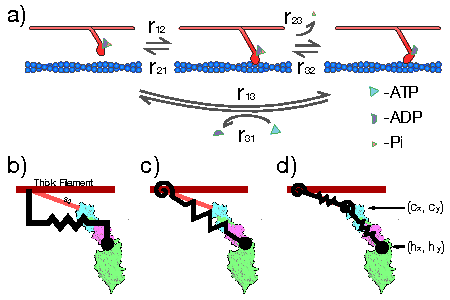
\includegraphics[width=3.2in]{../imgs/Figure1.pdf}
    \caption{
        \label{fig_xb_types}
        \textbf{Kinetic scheme and crossbridge types under investigation.} 
        The three state kinetic system is shown in subfigure a. 
        The three states represent (1) an unbound state, (2) a loosely bound state, and (3) a strongly bound state. 
        The binding rate ($r_{1,2}$), strong transition rate ($r_{2,3}$), and unbinding rate ($r_{3,1}$) are determined by the energy stored in the springs representing the crossbridge. 
        The reverse rates ($r_{2,1}$, $r_{3,2}$, and $r_{1,3}$) are functions of the forward transition rates.
        Subfigures b, c, and d show the representations of the crossbridge we examine, plotted against a myosin crystal structure for comparison. 
        Subfigure b shows the single-spring crossbridge (1sXB) used heavily used in models since \protect\citep{Huxley1957}. 
        Subfigure c depicts the two-spring crossbridge (2sXB) which uses both a torsional/angular spring and a linear spring. 
        Subfigure d shows a four-spring crossbridge (4sXB) using two torsional and two linear springs, which we compare the single and dual spring crossbridges against.
        The locations of the distal torsional spring and tip of the 4sXB are denoted as $(c_x, c_y)$ and $(h_x, h_y)$ respectively. 
        The tip of the 2sXB is also denoted as $(c_x, c_y)$.
    }
    \end{center}
\end{figure}

\begin{figure}[htbp]
    \begin{center}
    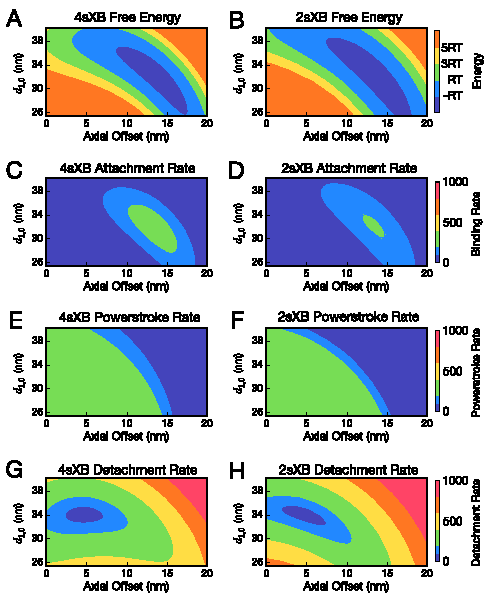
\includegraphics[width=3.2in]{../imgs/Figure2.pdf}
    \caption{
        \label{fig_kinetics_contours}
        \textbf{Energy and kinetics of the 4sXB and 2sXB systems at varying axial offsets and lattice spacings.} 
        Subfigures a through h show the properties of the 4sXB (subfigures a, c, e, and g) and the 2sXB (subfigures b, d, f, and h) as they change with binding site offset and $d_{1,0}$ lattice spacing.
        Binding site offset is the distance between the current axial location of the crossbridge's tip, $h_x$, and the location where the crossbridge attaches to the thick filament.
        Lattice spacing ($d_{1,-0}$) is defined as in \citet{Millman1998}, with an offset to account for filament thicknesses so that the crossbridge exactly bridges the two filaments at a rest lattice spacing of 34 nm.
        Subfigure a depicts the free energy of the 4sXB at various lattice spacings (represented along the y-axis), with the head stretched to an axial offset from the thick filament attachment point (zero on the x-axis).
        Similarly, the free energy of the 2sXB is shown in subfigure b.
        The lowest energy myosin head locations in both a and b are shown as the darkest part of the plot and change in axial offset as lattice spacing changes.
        The subfigures c and d show $r_{1,2}$, the probability that the 4sXB and the 2sXB will transition from an unbound state to a bound state, and the dependence of this transition on both the axial offset of the open binding site from the myosin thick filament attachment site and the lattice spacing $d_{1,0}$ which is a function of the distance between the binding site and the thick filament attachment point of the myosin head. 
        Subfigure c depicts this probability for the four spring crossbridge as a two dimensional contour with the same axes as a while subfigure d depicts the transition probabilities for the two spring crossbridge.
        Subfigures e and f show $r_{2,3}$, the probability of transition from a weakly bound state to a strongly bound state, for the same crossbridges, with the same axes and scales as c and d show $r_{1,2}$.
        Subfigures g and h show $r_{3,1}$, the probability of unbinding from a strongly bound state, for the same crossbridges, with the same axes and scales as c and d show $r_{1,2}$.
        The reverse rates, $r_{2,1}$, $r_{3,2}$, and $r_{1,3}$ may be back-calculated from the forward rates via the method described in \cite{Tanner:2007:pe115}.
    }
    \end{center}
\end{figure}

\begin{figure}[htbp]
    \begin{center}
    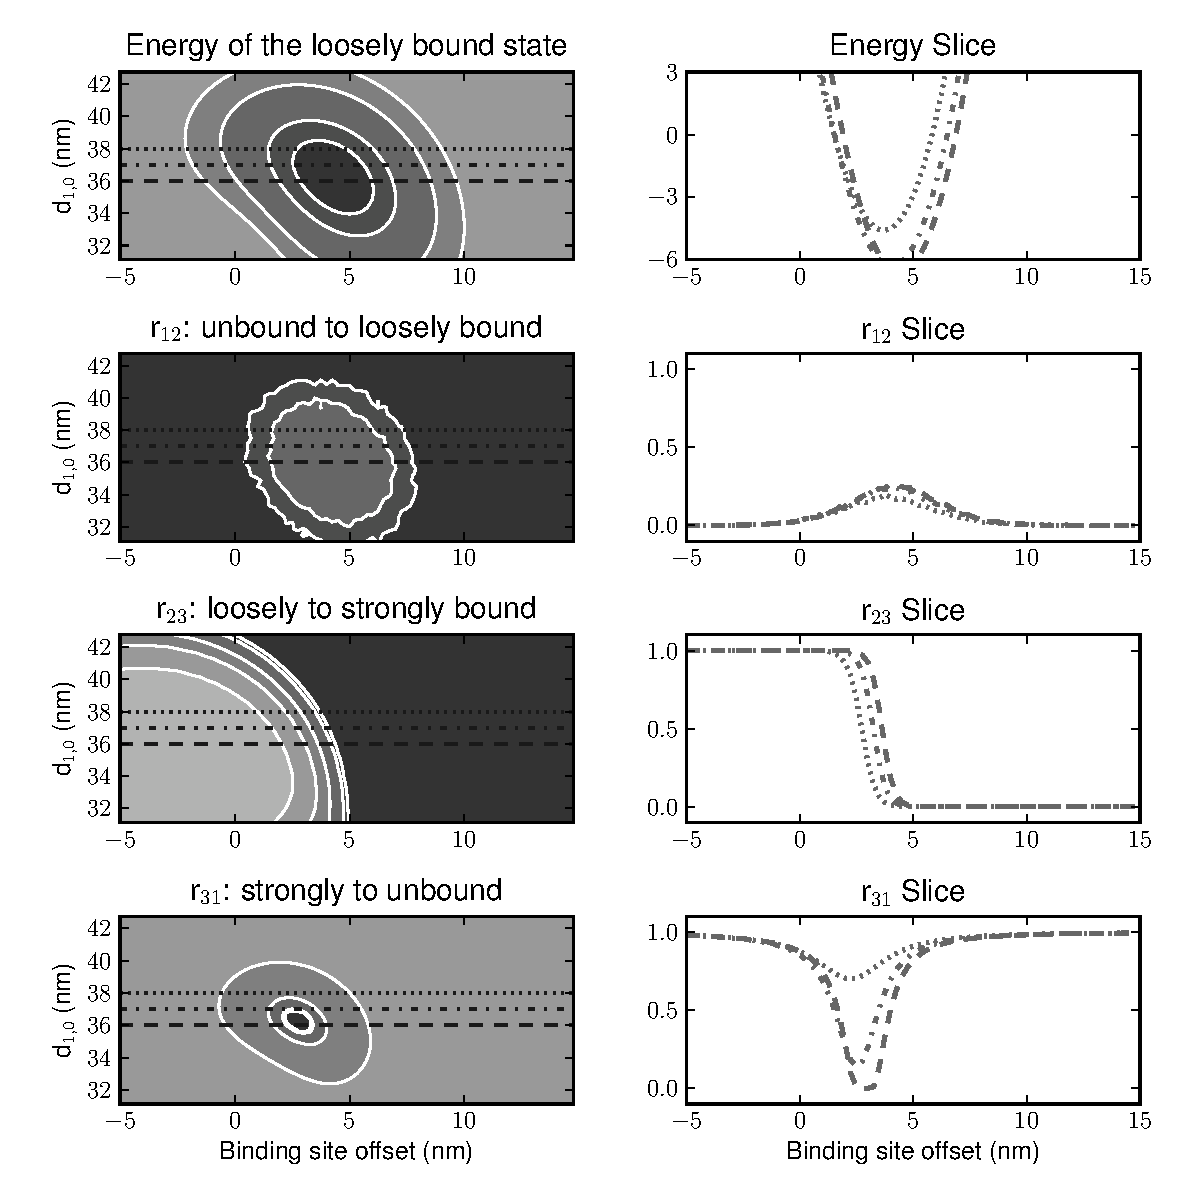
\includegraphics[width=3.2in]{../imgs/Figure3.pdf}
    \caption{
        \label{fig_kinetics_cuts}
        \textbf{Energy and kinetics of the 1sXB, 2sXB, and 4sXB at the resting lattice spacing.}
        Subfigures a through d show the energy and transition rates of the 1sXB (black line), 2sXB (green line), and 4sXB (red line) at resting lattice spacing.
        The 1sXB values shown for comparison are derived from those of \citet{Daniel1998} and \citet{Tanner:2007:pe115}, shifted axially so the resting location of the crossbridge head in each case is aligned with that of the 2sXB and 4sXB. 
        The free energy of the crossbridges in state two is shown in subfigure a, where the multi-spring crossbridges' shifts from a strictly parabolic trajectory is visible.
        The explicit thermal forcing of the multi-spring crossbridge heads in subfigure b results in binding probabilities that are more distributed than those of the single spring crossbridge.
        The rate of powerstrokes, in subfigure c, remains least changed between the single and the multi-spring crossbridge models.
        The energy-based kinetics of the multi-spring crossbridges are least able to replicate the detachment rated of the 1sXB, as shown in subfigure d. 
    }
    \end{center}
\end{figure}

\begin{figure}[htbp]
    \begin{center}
    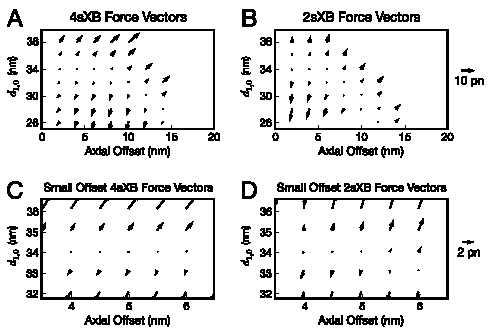
\includegraphics[width=3.2in]{../imgs/Figure4.pdf}
    \caption{
        \label{fig_forces}
        \textbf{Overview and detail of the forces exerted by the 2sXB and 4sXB.}
        Subfigures a through d show the forces exerted by the 4sXB and the 2sXB, with the shade of the vector arrows being determined by the chance of such a configuration occurring, a sum of the $r_{23}$ and \textbf{the} the inverse of the $r_{31}$ transition probabilities. 
        Subfigures e through h show, separated, the axial and radial components of the 4sXB and the 2sXB.
        Subfigures a and b show overviews of the forces exerted, respectively, by the 4sXB and the 2sXB over lattice spacings and axial offsets that vary as in Figure 2.
        The forces exerted by the two crossbridges have radial components which frequently equal or exceed their axial components.
        A more detailed view of the region surrounding the rest position of the crossbridges is shown in subfigures c and d, where the large radial components of the crossbridge forces, particularly for the 2sXB, is again evident.
    }
    \end{center}
\end{figure}

% \begin{figure}[htbp]
%     \begin{center}
%     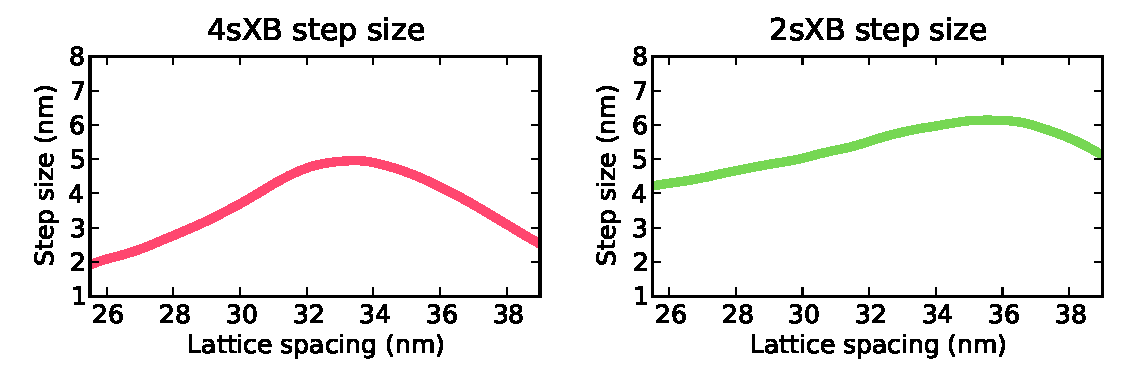
\includegraphics[width=3.2in]{../imgs/FigureS1.pdf}
%     \label{fig:one_spring_comparison}
%     \caption{
%         Comparison of traditional single spring crossbridge properties to those of the two spring crossbridge at resting lattice spacing.}
%     \end{center}
% \end{figure}
% 
% \begin{figure}[htbp]
%     \begin{center}
%     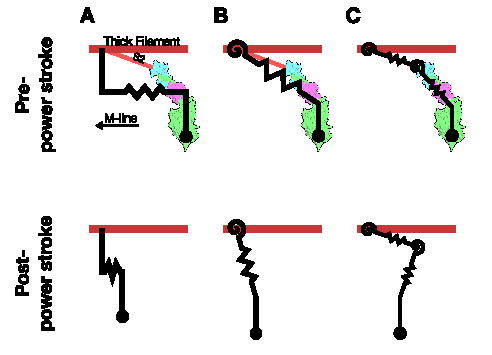
\includegraphics[width=3.2in]{../imgs/FigureS2.pdf}
%     \label{fig:force_components}
%     \caption{
%         Separated axial and radial components of force exerted by the two spring crossbridge at several lattice spacings.}
%     \end{center}
% \end{figure}

% section figures (end)



% bibliography (fold)
% Bib style requires biophysj.bst be in the document directory
\clearpage
\bibliographystyle{biophysj}
\bibliography{JournalArticles,NotArticles}
% bibliography (end)

\end{document}
